\documentclass{article}

\usepackage{color}
\usepackage[hidelinks]{hyperref}
\usepackage{url}
\usepackage[page]{appendix}
\usepackage[a4paper]{geometry}

\newcommand{\todo}[1]{\textbf{[[ TODO: }{\color{blue} #1}\textbf{]]}}
\newcommand{\fix}[1]{\textbf{[[ FIX: }{\color{red} #1}\textbf{]]}}

\newcommand{\eg}{\emph{e.g.}}
\newcommand{\ie}{\emph{i.e.}}

\newcommand{\jar}{\emph{jar}}
\newcommand{\ant}{Ant}
\newcommand{\maven}{Maven}
\newcommand{\gradle}{Gradle}
\newcommand{\sbt}{SBT}
\newcommand{\ivy}{Ivy}


\author{Jeanderson Barros Candido\\e-mail: \url{jeandersonbc@gmail.com}}
\title{Modernizing the Java PathFinder Build Workflow: Migrating from \ant{} to
\gradle{}}
\date{\today}

\begin{document}

\maketitle

\section*{Summary}

\noindent
Developers often perform recurrent tasks during the development process such
as testing, managing external libraries, generating API documentation, and
managing release artifacts.
Build tools help to automate those error-prone and daunt tasks.
Popular build tools usually provide a syntax to create a script file that
abstracts the commands to perform those tasks.
In the Java community, \ant{} used to be a popular choice but many
projects have been replacing it in favor of other modern builders.
\emph{This proposal aims to modernize the build workflow from the Java
PathFinder (JPF) project}.
To achieve this goal, I propose a smooth transitioning process to use
\gradle{}.
\gradle{} is a general purpose build system and uses Groovy, a JVM language, to
create and implement flexible and highly customizable build workflows.
This proposal enumerates the tasks and sets the expectations to ensure
successful collaboration by the end of the Google Summer of Code 2018 edition.

\section{Outline}
\label{sec:intro}

The JPF project currently uses \ant{} to automate the build workflow.
Unfortunately, \ant{} has drawbacks that hinder developer's productivity for
sufficiently complex and large projects.
In the context of the JPF project, there are two major issues:

\begin{enumerate}

\item \textbf{Lack of automatic dependency resolution.}
The user needs to manually download and configure dependencies.
\ant{} is often integrated with \ivy{}\cite{page:ivy} as a complementary
tool to handle external dependencies.
On the other hand, \gradle{}\cite{page:gradle} and \maven{}\cite{page:maven}
(and other popular build tools) resolve declared dependencies automatically
out-of-the-box.

\item \textbf{Large and verbose script file.}
XML has some drawbacks in the context of build automation.
Tags are often long names, and, in particular, \ant{} \emph{targets} may
contain several attributes and nested elements to describe additional
properties.
For sufficiently large projects, it is challenging to maintain and evolve the
build process due to the quick growth and the verbosity of the build script.

\end{enumerate}

Many popular build tools provide features to address those issues.
This proposal focuses on migrating from \ant{} to \gradle{}, and it is relevant
because the current JPF build workflow has error-prone processes that may
introduce barriers to newcomers willing to be part of the JPF community.
For further details on how and why I decided to migrate to \gradle{}, please,
refer to the Appendix~\ref{sec:eval}.

\section{Deliverables}
\label{sec:deliv}

\begin{itemize}
\item Gradle support on the \jpfcore{} module;
\item Gradle support on the \jpfsymbc{} extension module;
\item Updated version of the \texttt{jpf-template} auxiliary tool; 
\item Updated documentation related to the build process from the mentioned
projects;
\end{itemize}

\section{Strategy}
\label{sec:plan}

The main strategy to succeed with this proposal is to have a working \gradle{}
build since the beginning.
This is possible due to the interoperability of \ant{} withing a \gradle{}
execution~\cite{page:gradle-ant-support}.
Figure~\ref{fig:gradle-ant-support} demonstrates this feature with a simple
example: the \texttt{build.gradle} script imports a simple \texttt{build.xml}
file and the user can invoke the \texttt{hello} target as a \gradle{} task.

\begin{figure}[h!]
    \centering
    \begin{subfigure}[b]{0.4\textwidth}
        \lstinputlisting[title=\texttt{build.xml},language=XML]{snippets/ant-gradle-integration/build.xml}
    \end{subfigure}
    \hfill
    \begin{subfigure}[b]{0.4\textwidth}
        \lstinputlisting[title=Console output]{snippets/ant-gradle-integration/console.txt}
    \end{subfigure}
    \hfill
    \begin{subfigure}[b]{0.4\textwidth}
        \lstinputlisting[title=\texttt{build.gradle},language=Python]{snippets/ant-gradle-integration/build.gradle}
    \end{subfigure}
    \caption{Demonstration of \ant{} integration with
    \gradle{}.\label{fig:gradle-ant-support}}
    {\scriptsize Source: the author.}
\end{figure}

For this proposal, is not sufficient to only import the existing build script. 
The JPF core (\jpfcore) and Symbolic PathFinder (\jpfsymbc) modules have many
tasks and dependencies that could be simplified with a simpler and verifiable
syntax.
Figure~\ref{fig:tasks} illustrates the existing \ant{} targets and their
dependencies.
As we can see, critical paths involve mostly the compilation steps and must
be a priority since they represent the longer paths on the build workflow.
My strategy is to migrate each \ant{} target until the new build script
supports all original targets as \gradle{} tasks.
This is feasible because \gradle{} interchangeably handles \ant{} targets and
\gradle{} tasks.
Figure~\ref{fig:gradle-ant-dep} demonstrates the migration of an \ant{} target
to a \gradle{} task.
The \texttt{compile} target, originally on the \texttt{build.xml} file depends
on the \texttt{init} target and itself is a dependency to the \texttt{dist}
target.
After the migration, the \texttt{build.gradle} script imports the
\texttt{build.xml} and implements the \texttt{compile} task.
The new \gradle{} script performs the full build workflow despite being
incomplete.
This feature ensures that \ant{} and \gradle{} can coexist during the migration
process.

\begin{figure}[h!]
    \centering
    \begin{subfigure}[b]{0.75\textwidth}
        \centering
        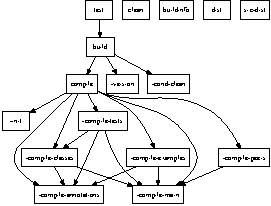
\includegraphics[width=.9\textwidth]{figs/jpf-tasks.pdf}%
        \caption{\jpfcore{}}
    \end{subfigure}
    \qquad
    \begin{subfigure}[b]{0.8\textwidth}
        \vspace{5mm}
        \centering
        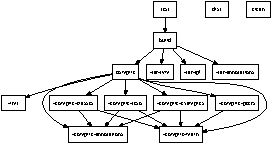
\includegraphics[width=\textwidth]{figs/symbc-tasks.pdf}%
        \caption{\jpfsymbc{}}
    \end{subfigure}
    \caption{\ant{} targets represented as directed acyclic graphs. The edges
    represent dependencies where the \emph{tail node} depends on the completion
    of the \emph{head node}.\label{fig:tasks}}
    {\scriptsize Source: the author.}
\end{figure}

\begin{figure}[h!]
    \centering
    \begin{subfigure}[b]{0.45\textwidth}
        \lstinputlisting[title=\texttt{build.xml},language=XML]{snippets/ant-gradle-dep/build-original.xml}
        \caption{Before migration}
    \end{subfigure}
    \hfill
    \begin{subfigure}[b]{0.45\textwidth}
        \lstinputlisting[title=\texttt{build.xml},language=XML]{snippets/ant-gradle-dep/build.xml}%
        \lstinputlisting[title=\texttt{build.gradle},language=python]{snippets/ant-gradle-dep/build.gradle}
        \caption{After migration}
    \end{subfigure}
    \caption{\ant{} and \gradle{} interoperability.\label{fig:gradle-ant-dep}}
    {\scriptsize Source: the author.}
\end{figure}

\section{Timeline}
\label{sec:time}

\fix{Missing tasks and constraints}

\subsection*{Community Bonding}
\event{Apr/23 - Apr/27}{\todo{...}}
\event{Apr/30 - May/04}{\todo{...}}
\event{May/07 - May/13}{\todo{...}}

\subsection*{Coding}
\subsubsection*{Phase 1}
\event{May/14 - May/20}{\todo{...}}
\event{May/21 - May/27}{\todo{...}}
\event{May/28 - Jun/03}{\todo{...}}
\event{Jun/04 - Jun/10}{\todo{...}}

\event{Jun/11 - Jun/15}{First Evaluation}

\subsubsection*{Phase 2}
\event{Jun/11 - Jun/17}{\todo{...}}
\event{Jun/18 - Jun/24}{\todo{...}}
\event{Jun/25 - Jul/01}{\todo{...}}
\event{Jul/02 - Jul/08}{\todo{...}}
\event{Jul/09 - Jul/13}{Second Evaluation}

\subsubsection*{Phase 3}
\event{Jul/09 - Jul/15}{\todo{...}}
\event{Jul/16 - Jul/22}{\todo{...}}
\event{Jul/23 - Jul/29}{\todo{...}}
\event{Jul/30 - Aug/05}{\todo{...}}
\event{Aug/06 - Aug/14}{Code submission and final evaluation}

\clearpage

\appendix
\section{Appendix}
\subsection{Build Tools Evaluation}
\label{sec:eval}

There are several build tools available in the Java community.
\maven{} and \gradle{} are two mainstream tools popular in Android and web
development.
\sbt{}\cite{page:sbt} is another build tool that is becoming popular, and it
was suggested in the GSOC idea's list\cite{page:jpf-gsoc18}.
Which one fits better to JPF's needs?
To answer this question, I evaluated \maven{}, \gradle{}, and \sbt{} in respect
to the following aspects:

\begin{itemize}
\item \emph{Q1. How are dependencies managed?} Configuring paths and \jar{}
files manually can be error-prone. Ideally, the build tool would take care of
paths and dependency versions automatically.
\item \emph{Q2. How brief and powerful is the build script format?} XML syntax
may lead to overly verbose and large files for sufficiently large projects.
Ideally, the chosen build tool offers a friendly and brief syntax and provides
an easy way to create user-defined tasks.

\end{itemize}

\subsubsection*{Results}
\label{sec:results}

\begin{itemize}
\item \emph{Answering Q1:}
One of the features introduced by \maven{} was the automatic management of
external dependencies.
By default, \maven{} fetches \jar{} files from the Maven Central
Repository\cite{page:mvncentral} and keep them locally.
In addition, \maven{} allows access to other repositories\cite{page:mvnrepo}
with minor configuration.
Not surprisingly, \gradle{} and \sbt{} not only adopted this feature but
\emph{are also compatible} with \maven{} repositories.
Therefore, \textbf{all options are tied in this question}.

\item \emph{Answering Q2:}
In this aspect, \maven{} inherits drawbacks from \ant{} since it is also based
on XML.
The major difference between \gradle{} and \sbt{} is the fact that their scripts not
only \emph{describe} the build process but also allow to specify \emph{how}
tasks can be performed.
Build scripts are actual code.
In the case of \sbt{} and \gradle{}, both are compatible with Java API.
This feature opens many possibilities and conveniences to create custom build
processes and user-defined tasks.
Therefore, \textbf{\sbt{} (Scala-based) and \gradle{} (Groovy-based) are both
valid options}.

\end{itemize}

\subsubsection*{Conclusion}
\maven{} is a mature tool with many advantages compared to \ant{}.
However, the build script lacks \emph{expressiveness} since it is also based on
XML.
\sbt{}, on the other hand, empowers the developer by specifying the build
process with real code.
In addition, Scala features interoperability with Java.
\sbt{} is a promising tool but it is relatively recent.
The first stable release is from February 9\textsuperscript{th},
2018\cite{page:sbt-release}.
\textbf{\gradle{} is a mature tool and combines the best of \maven{} and \sbt{}}
including features like incremental building, a daemon for efficient
execution\cite{page:gradle-daemon}, and also a convenient \emph{wrapper}
mechanism\cite{page:gradle-wrapper} for reproducible builds.
One of the most important \gradle{} features that support directly this
proposal is the interoperability with \ant{} build
scripts\cite{page:gradle-ant-support}\footnote{Section~\ref{sec:plan}
elaborates how this feature is used in this proposal}.
\textbf{For these reasons, \gradle{} seems to be a better fit for the context
of JPF.}
A list of useful links and snippets to demonstrate some \gradle{} basics are
available on GitHub\cite{page:gradle-labs} for further reference. 
Note that this evaluation is a sanity check and does not intend to be
generalized to all contexts in Java development.

\clearpage
\bibliographystyle{plain}
\bibliography{references}

\end{document}
